Un enseignant de grande section propose à ses élèves un jeu pour travailler la décomposition et la recomposition de nombres. Le jeu se compose de deux dés cubiques équilibrés et de corps de fourmis à compléter avec des pattes comme sur le dessin ci-dessous.

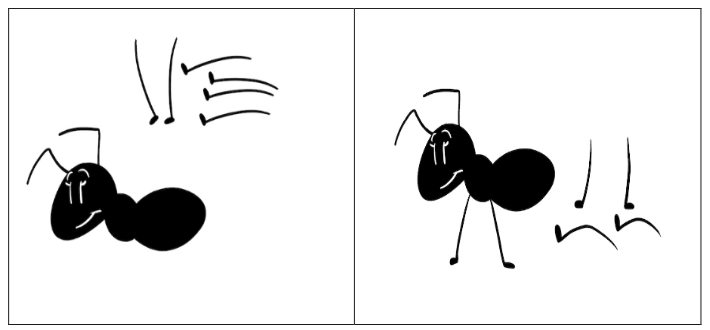
\includegraphics[width=.8\textwidth]{2022-g2-ex1-img1.png}

Sur les six faces du premier dé sont inscrits les nombres suivants : $1 ; 1 ; 2 ; 3 ; 4$ et $5 .$

Sur les six faces du deuxième dé sont inscrits les nombres suivants : $1 ; 2 ; 3 ; 4 ; 5$ et 5 .

On donne à chaque élève un corps de fourmi et 6 pattes à fixer sur le corps.

Au début de la partie, chaque élève choisit un nombre compris entre 2 et 10 . Ce nombre reste le même durant toute la partie. À tour de rôle, chaque élève joue. II lance les deux dés :

\begin{itemize}
  \item si la somme des nombres inscrits sur les faces supérieures des deux dés est égale au nombre choisi par cet élève, alors celui-ci fixe une patte à sa fourmi et relance les dés.

  \item sinon, c'est au joueur suivant de lancer les dés.

\end{itemize}
Il donne ensuite les dés au joueur suivant.

La partie se termine lorsqu'un élève a gagné, en fixant les six pattes de sa fourmi.

\begin{enumerate}
  \item Un élève choisit un nombre et lance les dés.
	\begin{enumerate}
		\item Quelles sont les différentes sommes qu'il peut obtenir ?
		\item Montrer que la probabilité qu'il obtienne 8 est égale à $\frac{4}{36}$.
	\end{enumerate}
  \item Un autre élève choisit le nombre 6 et lance les dés.
	\begin{enumerate}
		\item Quelle est la probabilité qu'il gagne une patte pour sa fourmi dès son premier lancer ?
		\item Quelle est la probabilité qu'il gagne deux pattes pour sa fourmi en 2 lancers ?
	\end{enumerate}
  \item Eden et Axelle commencent une partie. Eden choisit le nombre 6 et Axelle choisit un autre nombre.
	\begin{enumerate}
		\item Qui a le plus de chance de gagner la partie? Justifier.
		\item Eden est-il sûr de gagner la partie? Justifier.
	\end{enumerate}
\end{enumerate}